%Document-Author: Nicoletti Luca + Padovan Tommaso + Bortolazzo Matteo + Maino Elia + Bonato Paolo
%Document-Date: 2016/01/13
%Document-Description: Documento di Piano di qualifica

\documentclass[a4paper]{article}
\usepackage[english, italian]{babel}
\usepackage[T1]{fontenc}
\usepackage[utf8]{inputenc}
\usepackage{url}
\usepackage{graphicx}
\usepackage[hidelinks]{hyperref}
\usepackage{booktabs}
\usepackage{tabularx}
\usepackage{pifont}
\usepackage[table]{xcolor}
\usepackage{float}
\usepackage[]{appendix}
\usepackage{amsmath}
\usepackage{eurosym}
\usepackage{ltxtable}
\usepackage{geometry}

\geometry{margin=1in}

\graphicspath{{Immagini/}}

\newcolumntype{s}{>{\hsize=.21\hsize}X}
\newcolumntype{f}{>{\hsize=.37\hsize}X}
\newcolumntype{m}{>{\hsize=.42\hsize}X}


\newcolumntype{L}{>{\hsize=.3\hsize}X}
\newcolumntype{P}{>{\hsize=.125\hsize}X}



\renewcommand{\abstractname}{Tabella contenuti}

\begin{document}
	\begin{titlepage}
		% Defines a new command for the horizontal lines, change thickness here
		\newcommand{\HRule}{\rule{\linewidth}{0.5mm}} 
		\center  
		
		% HEADING SECTION
		\textsc{\LARGE SWEeneyThreads}\\[1.5cm] 
		\textsc{\Large Actorbase}\\[0.5cm] 
		\textsc{\large a NoSQL DB based on the Actor model}\\[0.5cm]
		
		
		% TITLE SECTION
		\HRule \\[0.4cm]
		{ \huge \bfseries Piano di qualifica}\\[0.4cm] 
		\HRule \\[1.5cm]
		
		% AUTHOR SECTION
		\begin{minipage}{0.4\textwidth}
			\begin{flushleft} \large
				\emph{Redattori:}\\
				Biggeri Mattia\\
				Tommasin Davide\\
			\end{flushleft}
		\end{minipage}
		~
		\begin{minipage}{0.4\textwidth}
			\begin{flushright} \large
				\emph{Approvazione:} \\
				\emph{Verifica:} \\
				Bonato Paolo \\
			\end{flushright}
		\end{minipage}
		
		%immagine
		\begin{figure}[H]
			\centering
			
\includegraphics[scale=0.8]{sweeney.png}
		\end{figure}
		\begin{center}
			Versione 1.1.8
		\end{center}
		% Date, change the \today to a set date if you want to be precise
		{\large \today}\\[3cm] 
		% Fill the rest of the page with whitespace
		\vfill  
	\end{titlepage}
	
	\tableofcontents
	\newpage
	\section*{Diario delle modifiche}
		\LTXtable{\textwidth}{Tabelle/tabelle_diario_modifiche/tabella_pdq.tex}
     
	\newpage
    \section{Introduzione}
		\subsection{Scopo del documento}
			Questo documento descrive le scelte effettuate in merito alle strategie 
			che il gruppo ha deciso di adottare per raggiungere obiettivi qualitativi e misurabili da 
			applicare al proprio prodotto. Per soddisfare questi obiettivi sarà necessario attuare un 
			processo di verifica continuo sulle attività svolte in modo da poter rilevare ed eventualmente 
			correggere anomalie e incongruenze in modo tempestivo per evitare danni e sprechi di risorse.
		\subsection{Scopo del prodotto}
			Il progetto consiste nella la realizzazione di un DataBase NoSQL key-value basato sul modello ad 
			Attori\ped{\textit{G}} con l'obiettivo di fornire una tecnologia adatta allo sviluppo di moderne 
			applicazioni che richiedono brevissimi tempi di risposta e che elaborano enormi quantità 
			di dati. Lo sviluppo porterà al rilascio del software sotto licenza MIT.
		\subsection{Glossario}
			Al fine di evitare ambiguità di linguaggio e di massimizzare la comprensione dei documenti, il 
	      gruppo ha steso un documento interno che è il \emph{Glossario v1.0.3}. In esso saranno definiti, in modo
	      chiaro e conciso i termini che possono causare ambiguità o incomprensione del testo.
		\subsection{Riferimenti}
			\subsubsection{Normativi}
				\begin{itemize}
					\item \textbf{Norme di progetto:} \\ \emph{Norme di progetto v1.1.1};
					\item \textbf{Capitolato d'appalto:} \\ \url{http://www.math.unipd.it/~tullio/IS-1/2015/Progetto/C1p.pdf}.
				\end{itemize}
			\subsubsection{Informativi}
				\begin{itemize}
					\item \textbf{Piano di progetto:} \\ \emph{Piano di progetto v1.0.4};
					\item \textbf{Slide del corso:} \\ \url{http://www.math.unipd.it/~tullio/IS-1/2015/};
					\item \textbf{SWEBOK - Version 3:} \\ \url{http://www.computer.org/web/swebok/v3};
					\item \textbf{\emph{TexMaker}:}\\ \url{http://www.xm1math.net/texmaker/};
				    \item \textbf{\emph{Scalastyle}:}\\ \url{https://github.com/scalastyle/scalastyle};
					\item \textbf{\emph{Scapegoat}:}\\ \url{https://github.com/sksamuel/scapegoat};
					\item \textbf{\emph{CLOC (Count Lines Of Code)}}:\\ \url{cloc.sourceforge.net};
					\item \textbf{\emph{ScalaTest}:}\\ \url{http://www.scalatest.org/}.
				\end{itemize}
	\section{Visione generale della strategia di verifica}
		
			\subsection{Definizione obiettivi}
			In questa sezione verranno descritti gli obiettivi di qualità relativi al prodotto che il 
			gruppo ha deciso di raggiungere e gli obiettivi relativi ai processi che saranno svolti per 
			il completamento del progetto.
			Per la stesura di questo documento e per la definizione delle metriche e degli strumenti atti a garantire la qualità del prodotto abbiamo seguito quanto definito in Appendice 4.5.1 e 4.5.2. 
	
\subsection{Misure e metriche}
			 Il processo di verifica, per avere un valore informativo, deve essere quantificabile e le misure rilevate
 devono essere basate su metriche stabilite a priori. 
 A causa della scarsa esperienza del gruppo, alcune metriche stabilite all'inizio potrebbero risultare approssimative ma
 seguendo il modello incrementale esposto nel \emph{Piano di progetto} si potrà migliorarne la precisione e l'accuratezza.

			Le tipologie di range ammesse sono due:
			\begin{itemize}
				\item \textbf{Accettabile:} Superiore al minimo valore richiesto affinché il prodotto sia accettato.
				\item \textbf{Ottimale:} Valori entro cui dovrebbe collocarsi la misurazione. Non sono vincolanti,
				ma fortemente consigliati. Misurazioni al di fuori di questi valori necessitano una verifica approfondita e nel
				caso non si trovi una maniera immediata per farli rientrare le cause di tale scostamento dovranno essere
				discusse nella successiva riunione.
			\end{itemize}
			\subsubsection{Metriche per i processi}
				Gli indici scelti per la quantificazione dei processi prendono in considerazione principalmente costi e tempi;
				hanno lo scopo di mantenere il controllo sui processi e che il progetto segua quanto descritto nel \emph{Piano di
				progetto}.
				
				Gli indici scelti sono:
				\begin{itemize}
					\item \textbf{SV (Schedule Variance):} É un indicatore di efficacia, mostra se si è o meno in linea con la
					pianificazione temporale rispetto alle attività nella baseline. Una schedule variance positiva indica che il
					gruppo è in anticipo rispetto al Piano di progetto, che è in ritardo altrimenti.
					\item \textbf{BV (Budget Variance):} Indica se la spesa sostenuta alla data corrente è superiore o inferiore a
					quella preventivata. Una budget variance positiva indica che si è speso meno di quanto inizialmente previsto,
					viceversa altrimenti.		
				\end{itemize}
				
				
			\subsubsection{Metriche per i documenti}
				Per i documenti abbiamo scelto di adottare le seguenti metriche: 
				
				\begin{itemize}
				\item \textbf{Gulpease:} Lo abbiamo scelto come \emph{indice di leggibilità} in quanto:
				\begin{itemize}
					\item È l'unico tarato appositamente per la lingua italiana.
					\item Utilizza la lunghezza delle parole in lettere anziché in sillabe, quindi è più semplice da automatizzare
					\item Considera la lunghezza della parola e la lunghezza della frase rispetto al numero delle lettere
					\item Permette di misurare la complessità dello stile di un documento
				
				\end{itemize}
				La formula per il suo calcolo è la seguente:
				\begin{align}
					89+\frac{300\cdot(numero\ delle\ frasi)-10\cdot(numero\ delle\ lettere)}{numero\ delle\ parole}
				\end{align}
				
				I risultati sono compresi tra 0 e 100, dove il valore "100" indica la leggibilità più alta e "0" la leggibilità
				più bassa. In generale risulta che testi con un indice
				\begin{itemize}
					\item inferiore a 80 sono difficili da leggere per chi ha la licenza elementare
					\item inferiore a 60 sono difficili da leggere per chi ha la licenza media
					\item inferiore a 40 sono difficili da leggere per chi ha un diploma superiore
				\end{itemize}
	
				Il gruppo si atterrà ai seguenti parametri:
				\begin{itemize}
					\item Range di accettazione: [35|100]
					\item Range di ottimale: [45|100]
				\end{itemize}
				\item \textbf{Numero parole:} Questa metrica servirà principalmente per misurare l'incremento del documento durante il completamento delle varie fasi.
				\item \textbf{Numero figure e tabelle su numero pagine:} Questa metrica verrà valutata solamente su i documenti esterni per verificarne la difficoltà di lettura.
				Il gruppo si atterrà ai seguenti parametri:
				\begin{itemize}
					\item Range di accettazione: [0,25|2]
					\item Range di ottimale: [0,5|2]
				\end{itemize}
				\item \textbf{Media parole per section:} Servirà ad evitare la costruzione di sezioni troppo grandi, in modo che tutti
				gli argomenti siano facilmente trovabili sull'indice.
				\begin{itemize}
					\item Valori accettati: [100|250]
					\item Valori ottimali: [0|100]
				\end{itemize}
				\item \textbf{Numero di errori ortografici:} 
				Garantisce l'assenza di errori ortografici rilevati dal correttore automatico, a meno di falsi positivi.
				\begin{itemize}
					\item Range di accettazione: [0|0]
					\item Range di ottimale: [0|0]
				\end{itemize}
				
				\item \textbf{Livelli di annidamento dei requisiti:}
				Misura i livelli degli alberi dei requisiti. In questo modo si vuole dare una stima di quanto essi
				siano organizzati gerarchicamente.
				\begin{itemize}
					\item Valori accettati: da decidere
							\item Valori ottimali: da decidere
				\end{itemize}
				
			\end{itemize}
				
				
				
			
			\subsubsection{Metriche per il software}
				Questa sezione è da intendere come una dichiarazione di intenti e probabilmente verrà rivista quando inizieremo 
				realmente la fase di programmazione.

				Al fine di perseguire gli obbiettivi sulla qualità del software, applicheremo le seguenti metriche:
				\begin{itemize}
					\item \textbf{Attributi per classe:}
						Un grande numero di attributi interni ad una classe mostra probabilmente la necessità di suddividere la classe 
						in più classi relazionate tra loro.
						\begin{itemize}
							\item Valori accettati: [0|18]
							\item Valori ottimali: [2|9]
						\end{itemize}

					\item \textbf{Numero livelli annidamento:}
						Mostra il livello di annidamento dei metodi, un numero alto implica una bassa astrazione del codice ed 
						un' elevata complessità.
						\begin{itemize}
							\item Valori accettati: [1|8]
							\item Valori ottimali: [1|4]
						\end{itemize}

					\item \textbf{Numero parametri per metodo:}
						Un valore elevato indica che probabilmente il metodo ha un sovraccarico di funzionalità.
						\begin{itemize}
							\item Valori accettati: [0|8]
							\item Valori ottimali: [0|5]
						\end{itemize}

					\item \textbf{Linee di codice per linee di commento:}
						È la percentuale di righe di commento rispetto al totale delle righe di codice. Utile per la manutenibilità.
						\begin{itemize}
							\item Valori accettati: [0,2|0,7]
							\item Valori ottimali: [0,3|0,5]
						\end{itemize}

					\item \textbf{Accoppiamento afferente:}
						Indica il numero di classi esterne ad un package che dipendono da esso, un grande valore indica una forte 
						dipendenza del software per il package in questione, un valore basso invece indica una bassa utilità del 
						package per il resto del software.
						\begin{itemize}
							\item Valori accettati: da decidere
							\item Valori ottimali: da decidere
						\end{itemize}

					\item \textbf{Accoppiamento efferente:}
						Il numero di classi di un package che dipendono da package esterni, un valore basso indica che il package ha 
						numerose funzionalità indipendenti dal resto del software.
						\begin{itemize}
							\item Valori accettati: da decidere
							\item Valori ottimali: da decidere
						\end{itemize}
						
					\item \textbf{Linee di codice per metodo:}
						È una misura della leggibilità del codice: valori troppo elevanti indicano che il corpo di un metodo
						potrebbe essere scarsamente comprensibile.
						\begin{itemize}
							\item Valori accettati: da decidere
							\item Valori ottimali: da decidere
						\end{itemize}
						
					\item \textbf{Source Line Of Code (SLOC):}
						Il numero di istruzioni presenti nel codice. Questa metrica fornisce una stima della complessità del programma.
						È utile anche per dare una stima di quanto il codice incrementerà nel tempo, semplificando così la
						pianificazione.
						\begin{itemize}
							\item Valori accettati: da decidere
							\item Valori ottimali: da decidere
						\end{itemize}
					
					\item \textbf{Complessità Ciclomatica:}
						Una metrica sviluppata da Thomas J. McCabe che consente di stimare la complessità di un programma misurando
						il numero di cammini linearmente indipendenti attraverso il grafo di controllo di flusso.
						\begin{itemize}
							\item Valori accettati: da decidere
							\item Valori ottimali: da decidere
						\end{itemize}
					
					
					
			\end{itemize}
			
			
		\subsection{Strumenti e metodi per l'applicazione delle metriche}
			Le risorse software che si utilizzeranno durante il processo di verifica sono:
			\begin{itemize}
				\item \textbf{\emph{TexMaker}:} un ambiente grafico Open-Source per \LaTeX cross-platform, permette 
				la compilazione rapida e la visualizzazione del PDF generato, sarà anche usato per il controllo ortografico;
				\item \textbf{\emph{Scalastyle}:} analizzatore statico che rileva potenziali problemi nel codice, da utilizzare sia durante la produzione del codice, sia durante la sua verifica
				 (\url{https://github.com/scalastyle/scalastyle});
				\item \textbf{\emph{Scapegoat}:} un altro analizzatore statico che si concentra maggiormente sugli 
				standard di stile e di coding (\url{https://github.com/sksamuel/scapegoat});
				\item \textbf{\emph{CLOC (Count Lines Of Code)}:} misura alcune metriche riguardanti il codice 
				sorgente in vari linguaggi, tra cui \emph{Scala}, servirà a calcolare le linee di codice per linee di commento (\url{cloc.sourceforge.net});
				\item \textbf{\emph{ScalaTest}:} framework per i test su Scala (\url{http://www.scalatest.org/}).
				
				\item \textbf{Repo's Outpost:} tool su piattaforma web sviluppato dai componenti del gruppo,
				disponibile (previo login) all'indirizzo: \\
				\url{http://sweeneytreadaas.altervista.org/menuPrincipale/documentation_tools/documenti_latex.php} \\
				Fornisce una \emph{dashboard} aggiornata in tempo reale che riporta le principali
				metriche dei documenti presenti nel repository.
				I valori sono evidenziati con diversi colori che ne caratterizzano ottimalità,
				accettabilità o non accettabilità.
				%immagine
				\begin{figure}[H]
					\centering
					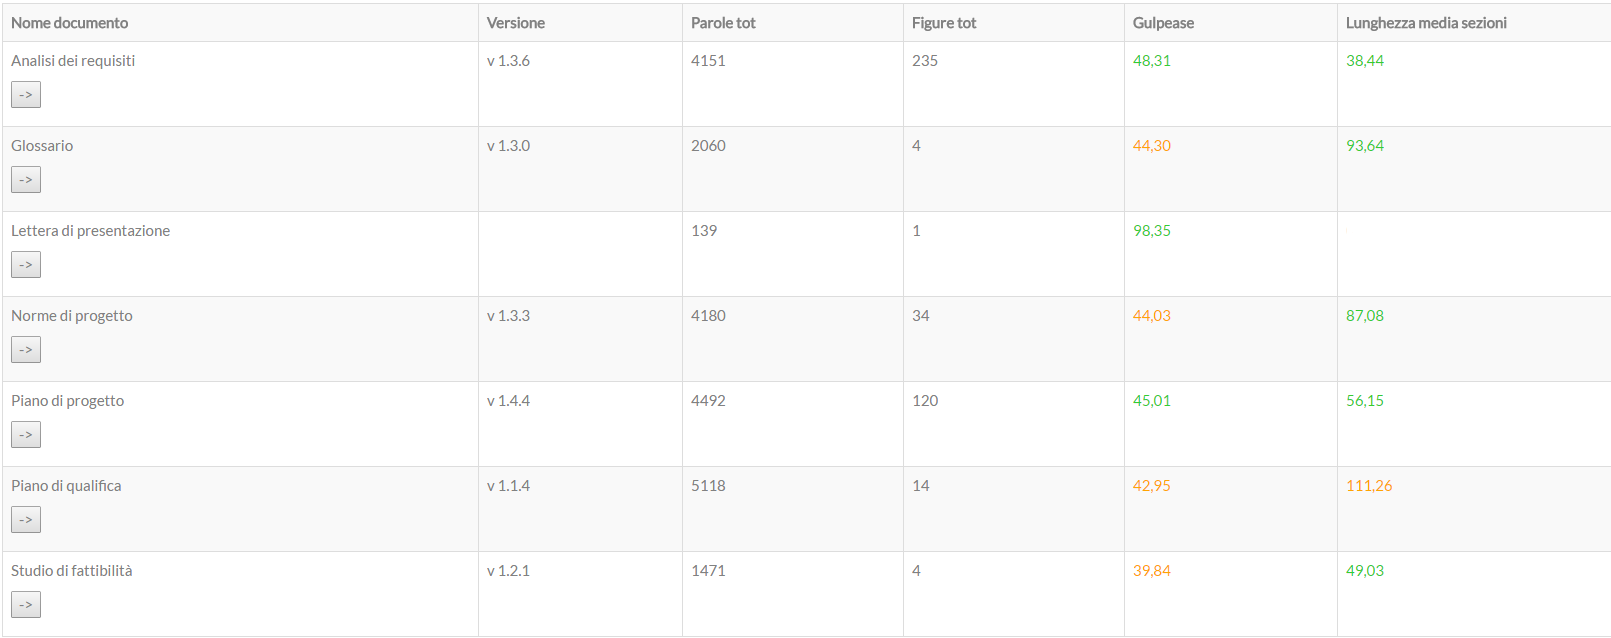
\includegraphics[scale=0.35]{immagini/Pdq/repoOutpost.png}
					\caption{Screenshot del tool Repo's Outpost}
				\end{figure}
				
				\item \textbf{Camel Calculator:} tool su piattaforma web sviluppato dai componenti del gruppo,
				disponibile (previo login) all'indirizzo: \\
				\url{http://sweeneytreadaas.altervista.org/menuPrincipale/documentation_tools/metric_calc.php} \\
				Permette di calcolare nel dettaglio le metriche di uno specifico documento. È possibile caricare
				il file mediante diverse modalità, compresi dei link diretti per i documenti nel repository del gruppo.
				
				\item \textbf{Gloss Buddy:} tool su piattaforma web sviluppato dai componenti del gruppo,
				disponibile (previo login) all'indirizzo: \\
				\url{http://sweeneytreadaas.altervista.org/menuPrincipale/documentation_tools/glossario.php} \\
				Marca i termini del glossario con la simbologia corretta.
				
			\end{itemize}
		\subsection{Metodi}
			
			\subsubsection{Analisi dei processi}
				I processi compiuti durante una fase verranno analizzati secondo il seguente protocollo:
				\begin{itemize}
					\item \textbf{Controllo delle metriche:}
						Alla conclusione di ogni fase del progetto si calcolano gli indici definiti nella sezione 2.2.1 confrontando 
						le macro-attività preventivate nel \emph{Piano di progetto} con i dati effettivi riscontrati dal sistema di ticketing.
					\item \textbf{Analisi PDCA:}
						Secondo il ciclo PDCA una fase di progetto ha inizio con la pianificazione di come possono essere migliorati i processi. 
						Durante la fase vengono attuati i cambiamenti prefissati e alla fine viene effettuato un controllo. Se un processo 
						risulta essere migliore viene adottato in modo definitivo, se invece risulta inalterato o addirittura peggiore i 
						cambiamenti vengono scartati.
				\end{itemize}
			\subsubsection{Analisi dei documenti}
				Ogni documento redatto è verificato mediante il seguente protocollo:
				\begin{itemize}
					\item \textbf{Controllo sintattico:} Il testo deve venire sottoposto a controllo dell'ortografia con il tool
					fornito dall'ambiente di sviluppo \LaTeX utilizzato. Alcuni errori non possono essere comunque rilevati da
					meccanismi automatici, quindi al fine di ottenere correttezza sintattica e semantica i Verificatori
					effettueranno un walkthrough al fine di ricercare errori sfuggiti al correttore ortografico.
					\item \textbf{Controllo semantico:}
		I Verificatori sono tenuti a leggere il documento, controllando che le frasi lette abbiano
		senso compiuto e che siano pertinenti all'argomento trattato nella sezione. Errori di questo
		tipo possono essere dovuti a sviste o errori di copia nella stesura.
					\item \textbf{Rispetto delle Norme di progetto:} I Verificatori sono tenuti a verificare che il documento
					rispetti tutte le norme tipografiche e di struttura del documento riportate nelle \emph{Norme di progetto}. Porzioni
					di questa verifica sono automatizzabili, i Verificatori dovranno quindi usare tool ove possibile. 
					\item \textbf{Inspection secondo checklist:} I Verificatori dovranno scorrere la lista di controllo e
					verificare che non sia presenti gli errori comuni lì riportati.
					\item \textbf{Verifica Glossario:} I Verificatori dovranno controllare che tutti i termini contenuti nel 
					Glossario siano indicati all'interno dei documenti con la G a pedice. 
					\item \textbf{Calcolo delle metriche:} I Verificatori dovranno calcolare le seguenti metriche per ogni documento:
					\begin{itemize}
						\item \textbf{Gulpease:}I verificatori calcoleranno l'indice Gulpease del documento tramite strumenti automatici forniti su \url{http://sweeneytreadaas.altervista.org/menuPrincipale/documentation_tools/}, in caso i risultati non siano soddisfacenti presenterà al redattore le sezioni peggiori;
						\item \textbf{Numero figure e tabelle su numero pagine:}Tramite gli elenchi delle figure e delle tabelle sarà calcolato il rapporto tra la somma delle stesse e il numero di pagine, e se risulterà scadente il verificatore lo segnalerà al redattore del documento.
						\item \textbf{Media parole per section:}La metrica sarà calcolata tramite strumenti automatici e in caso di valori non accettabili le sezioni peggiori saranno comunicate al redattore.
					\end{itemize}
					\item \textbf{Miglioramento:} Se nello svolgimento di uno qualunque dei punti precedenti un Verificatore
					notasse nuove possibilità di automatizzazione dovrà segnalarle e si dovrà cercare o costruire uno strumento per
					rendere effettiva tale automatizzazione. Inoltre durante le esecuzioni dei walkthrough, i verificatori sono
					tenuti ad annotare gli errori più frequenti o potenzialmente dannosi rilevati. Tali errori andranno poi ad
					aggiornare la lista di controllo che verrà utilizzata per le successive inspection.
				\end{itemize}		
		\subsection{Organizzazione}
			Il processo di verifica inizia fin dal primo rilascio ufficiale nella repository di un documento vX.0.0, il risultato 
			del processo di verifica cambia la versione del documento, incrementandone la versione al secondo livello di profondità, 
			il documento quindi passa a vX.1.0. Ogni modifica apportata al documento ne aumenta la versione all'ultimo livello di 
			profondità. Una volta completate le modifiche e le verifiche continue sui documenti, esso passa nella fase di validazione,
			a carico del responsabile, che ne fa cambiare la versione al secondo livello di priorità. 
			
			Come descritto nelle \emph{Norme di progetto}, il primo valore in una versione verrà cambiato ad ogni consegna.
			
			Grazie al diario delle modifiche è più facile individuare dove concentrare l'attenzione nelle verifiche successive 
			alla prima, in quanto sono segnate le sezioni che sono state aggiunte o che hanno subito dei cambiamenti dall'ultima
			 verifica, evitando cosi di controllare sempre tutto il documento ad ogni rilascio di versione, per cui ottimizzando 
			 il tempo necessario al controllo.

			Per ognuna delle 5 fasi del progetto descritte nel \emph{Piano di Progetto v 1.0.5}, sono necessarie diverse attività 
			di verifica a causa dei diversi output ottenuti:

			\begin{itemize}
				\item \textbf{Analisi:} Si devono seguire le attività di verifica descritte nella sezione 2.9.2 e 2.9.1 sui processi 
				e sui documenti attuati.
			\end{itemize}
			
			Come detto in precedenza conclusa la verifica, ha inizio il processo di approvazione. Durante questo processo è compito 
			del Responsabile di Progetto accertarsi che i prodotti ottenuti siano conformi a quanto pianificato e progettato.
		
		
		\subsection{Pianificazione strategica e temporale}
			Avendo lo scopo di rispettare le scadenze riportate nel \emph{Piano di progetto}, è necessario che l'attività 
			di verifica, sia del codice che della documentazione, sia sistematica e ben organizzata; in questo modo 
			l'individuazione, e quindi la correzione degli errori avverrà il prima possibile, limitando la diffusione 
			degli stessi.\\
			Per cercare di ridurre il numero degli errori, e quindi semplificare l'attività di verifica, ogni fase 
			di codifica o documentazione sarà preceduta da una fase di studio preliminare. Evitando le imprecisioni 
			di natura concettuale si ridurranno le correzioni necessarie.
			
			Di seguito vengono riportate le scadenze previste:
			\begin{itemize}
				\item \textbf{Revisione dei requisiti:} 2016-01-22;
				\item \textbf{Revisione di progettazione:} 2016-04-18;
				\item \textbf{Revisione di qualifica:} 2016-05-23;
				\item \textbf{Revisione di accettazione:} 2016-06-17.
			\end{itemize}
		\subsection{Responsabilità}
			Il \emph{Responsabile di progetto} ha il compito di:
			\begin{itemize}
				\item Accertarsi che le attività di verifica vengano svolte sistematicamente secondo quanto 
				riportato nelle \emph{Norme di progetto};
				\item Accertarsi che vengano rispettati ruoli e competenze assegnate nel \emph{Piano di progetto};
				\item Verificare che non ci siano conflitti di interesse tra redattori e \emph{Verificatori};
				\item Aprire ed assegnare i ticket principali e le task-list;
				\item Approvare un documento e sancirne la distribuzione.
			\end{itemize}
			I \emph{Verificatori} hanno il compito di:
			\begin{itemize}
				\item Effettuare la verifica dei documenti con strumenti e metodi proposti nel \emph{Piano di Qualifica};
				\item Attenersi rigidamente a quanto sancito nelle \emph{Norme di progetto};
				\item Segnalare tempestivamente un errore, qualora riscontrato;
				\item Sottoporre i documenti all'approvazione del \emph{Responsabile}, una volta giunti ad uno stadio finale.
			\end{itemize}
		\subsection{Risorse}
			Per la realizzazione del progetto sono necessarie risorse sia umane che tecnologiche.
			\subsubsection{Risorse umane}
				Vengono descritte nel dettaglio nel \emph{Piano di progetto} e sono:
				\begin{itemize}
					\item \emph{Responsabile di progetto};
					\item \emph{Amministratore};
					\item \emph{Analista};
					\item \emph{Progettista};
					\item \emph{Programmatore};
					\item \emph{Verificatore}.
				\end{itemize}
			\subsubsection{Risorse software}
				Sono necessari tutti i software utili
				\begin{itemize}
					\item alla gestione di documentazione in \LaTeX;
					\item alla creazione di diagrammi UML;
					\item allo sviluppo di codice \emph{Scala};
					\item a semplificare ed automatizzare la verifica;
					\item a semplificare ed automatizzare la pianificazione e la documentazione della stessa;
					\item a semplificare ed automatizzare la comunicazione interna tra i membri del gruppo;
					\item a gestire test ed analisi sul codice.
				\end{itemize}
				\subsubsection{Risorse hardware}
					\begin{itemize}
						\item computer dotati di tutti i software descritti nel \emph{Piano di qualifica} e nelle
						\emph{Norme di progetto};
						\item luoghi dove effettuare le riunioni del gruppo.
					\end{itemize}
				Tutti i membri del gruppo hanno a disposizione almeno un computer personale dotato di tutti gli strumenti
				necessari per il progetto; tutte le macchine in questione sono portatili. Inoltre in caso di rottura o guasto
				è messo a disposizione un computer di riserva. Sono a disposizione quattro appartamenti a Padova dove
				effettuare le riunioni. La scelta di quale viene presa di volta in volta a seconda delle disponibilità. Tutti
				gli appartamenti sono dotati di connessione internet a banda larga.				
				

		\subsection{Analisi}
			\subsubsection{Tecniche per l'analisi statica}
				L'analisi statica non richiede l'esecuzione del codice in oggetto, ed è quindi applicabile sia 
				alla documentazione che al codice. Permette di individuare errori ed anomalie al più presto possibile, 
				scongiurandone la diffusione. \\ Essa può essere svolta in due modi distinti.
				\subsubsection{Walkthrough}
					Si svolge effettuando una lettura critica a pettine. Questa tecnica viene utilizzata prevalentemente 
					nelle prime fasi del progetto, in cui non si ha ne una adeguata esperienza, ne uno storico degli errori 
					più comuni che permetta una indagine più mirata. I Verificatori, tramite questa tecnica, saranno in 
					grado di stilare una lista di errori più frequenti, potendo così applicare successivamente la tecnica 
					\emph{Inspection}. Il \emph{Walkthrough} è una tecnica onerosa e richiede l'intervento di più persone. 
					Dopo una fase iniziale in cui i Verificatori leggono il documento ed individuano potenziali errori essi 
					devono essere discussi in una riunione con altri componenti del gruppo per accertare che non siano dei 
					falsi positivi.
				\subsubsection{Inspection}
					È una tecnica molto meno onerosa. Consiste nel controllare alcune parti dei documenti che si sono rivelate 
					maggiormente prone ad errori. Per ottenere questo risultato è necessario avere una lista di controllo che 
					indichi quali sono le parti da controllare in maniera mirata. Essa viene stilata durante le fasi di 
					\emph{Walkthrough}. Un altro motivo per cui la \emph{Inspection} è preferibile è il fatto che essa richiede 
					l'intervento dei soli verificatori, che poi possono procedere alla correzione della maggior parte degli errori, 
					oppure ad aprire un ticket riguardante quelli che non sono di immediata risoluzione.\\
					
					
				Durante l'applicazione del \emph{Walkthrough} ai documenti sono state riportate le tipologie di errori più frequenti, 
				esse costituiscono quindi la lista di controllo per le verifiche ad \emph{Inspection},
				l'attuale lista si trova in appendice sezione 4.6 e una versione sempre aggiornata della stessa è presente sul drive del gruppo.
				
			\subsubsection{Tecniche per l'analisi dinamica}
				Questo tipo di analisi richiede una esecuzione di parte del programma, quindi ovviamente non applica 
				ai documenti ma solo al codice. Il suo obiettivo è rilevare errori o difetti di implementazione 
				mediante l'uso di test che devono essere necessariamente ripetibili: solo un test che produca lo 
				stesso output partendo dallo stesso ambiente e lo stesso input può è capace di riscontrare problemi. 
				L'attore che esegue un test deve definire a priori ed avere il pieno controllo su:
				\begin{itemize}
					\item \textbf{Ambiente:} insieme di hardware a software come sistema operativo e altri programmi o 
					processi in esecuzione;
					\item \textbf{Specifiche:} definizione degli input e dei relativi output attesi, che sono ripetibili 
					in quanto si postula di essere in un ambiente deterministico;
					\item \textbf{Procedure:} descrizione delle azioni compiute dall'attore (umano o computer che sia) 
					per arrivare allo stato iniziale, far partire l'esecuzione, inserire gli input specificati e verificare 
					che l'output sia uguale a quello atteso.
				\end{itemize}
				
				Sono definiti 5 tipi di test:
				\begin{itemize}
					\item \textbf{Test di unità:} Una unità viene definita come la più piccola quantità di software che conviene
					testare singolarmente. Il fine di questi test è cercare di individuare eventuali errori presenti nelle singole
					unità che compongono l'intero sistema. Essi vengono testati attraverso l'uso di stub, driver e logger. Queste
					verifiche sono spesso le più onerose, ma anche quelle che portano alla luce il maggior numero di errori, quindi
					quelle che producono il maggior valore.
					\item \textbf{Test di integrazione:} Consiste nella verifica di componenti del sistema che vengono aggiunti
					incrementalmente, è necessario dunque analizzare combinazioni di due o più unità di software. Hanno lo scopo di
					individuare errori residui nella realizzazione dei singoli moduli, modifiche delle interfacce e comportamenti
					inaspettati di componenti software preesistenti forniti da terze parti che non si conoscono a fondo. Per la
					loro realizzazione è necessario usare spesso componenti fittizie non ancora sviluppate, ma che emulano il
					comportamento atteso.
					\item \textbf{Test di Sistema:} Consiste nella validazione del prodotto software una volta che siano stati
					aggiunti tutti i componenti e lo si ritiene giunto ad una versione definitiva. Lo scopo principale è verificare
					che ci sia totale copertura dei requisiti stabiliti nella fase di Analisi di dettaglio. È obiettivo
					fondamentale della qualità del processo fare in modo che giunti a questo punto l'esito del test sia comunque
					positivo, in quanto garantito dal tracciamento dei requisiti.
					\item \textbf{Test di regressione:} Consiste nell'eseguire nuovamente i test di unità e integrazione in
					porzioni di software che hanno subito modifiche in maniera da accertare che questi cambiamenti non
					pregiudichino il funzionamento dei componenti non toccati da questa modifica.
					\item \textbf{Test di accettazione:} Consiste nel collaudo del prodotto che viene eseguito in presenza del
					proponente. Un esito positivo di questo test permette il rilascio ufficiale del software.
					
				\end{itemize}
				
										
			
	\section{Gestione amministrativa della revisione}
		\subsection{Comunicazione e risoluzione di anomalie}
			Una anomalia è una violazione da parte di un documento, o unità di codice, di una o più delle seguenti condizioni:
			\begin{itemize}
				\item Conformità alla norme tipografiche o di codifica;
				\item Appartenenza al range di accettabilità per tutte le metriche descritte nella \emph{Sezione 2};
				\item Congruenza del prodotto con funzionalità indicate nell'\emph{analisi dei requisiti};
				\item Congruenza del codice con il design del prodotto.
			\end{itemize}
			Se un \emph{Verificatore} dovesse trovare una anomalia egli è tenuto ad aprire un sotto-ticket all'interno 
			della task-list a lui assegnata. Nel caso la risoluzione del ticket avesse la necessità di essere strutturato 
			in sotto-attività sarà compito del \emph{Responsabile} aprire una nuova task-list ed assegnarla alle figure coinvolte.

		\subsection{Procedure di controllo qualità per i processi}
			La qualità del processo viene garantita da:
			\begin{itemize}
				\item \textbf{Pianificazione:} i processi devono essere pianificati nel dettaglio, in maniera da determinare 
				i punti e le tempistiche in cui effettuare controlli;
				\item \textbf{Controllo:} i controlli pianificati devono essere eseguiti in maniera oggettiva e neutrale, 
				quindi con strumenti automatici ovunque possibile;
				\item \textbf{Miglioramento continuo:} l'adozione del principio di \emph{PDCA} aiuterà a migliorare i processi durante l'intera durata del progetto..
			\end{itemize}
		\subsection{Procedure di controllo qualità per il prodotto}
			La qualità del prodotto viene garantita da:
			\begin{itemize}
				\item \textbf{Comprensione ed analisi del dominio};
				\item \textbf{Verifica:} determina che l'output di una fase sia consistente, completo e corretto. 
				Deve essere eseguita costantemente per tutta la durata del progetto, ma cercando di essere minimamente invasiva;
				\item \textbf{Validazione:} conferma oggettivamente che il prodotto sia conforme alle aspettative;
				\item \textbf{Quality Assurance:} garantisce il raggiungimento degli obiettivi di qualità, in maniera preventiva. 
				In questo modo si riduce drasticamente il ricorso a tecniche retrospettive, e con esse si riducono le iterazioni.
			\end{itemize}
		\section{Appendice}
			\subsection{Qualità}
Riportiamo gli standard di riferimento per sviluppare le metriche e i metodi atti a garantire la qualità del prodotto.
				\begin{figure}[H]
					\centering
					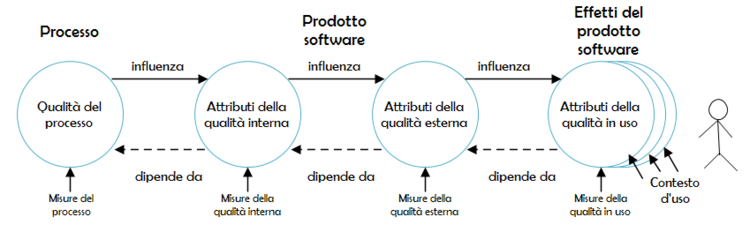
\includegraphics[scale=0.65]{immagini/Pdq/QualitaDelProdottoSoftware.PNG}
					\caption{Influenze e dipendenze delle varie misure di qualità.}
				\end{figure}
			\subsubsection{Qualità di processo}
				Per garantire la qualità del prodotto è necessario garantire anche quella dei processi necessari 
				al suo completamento. A questo scopo si è deciso di adottare lo standard 
				ISO/IEC 15504 denominato SPICE.
				
				Questo modello descrive come ogni processo debba essere controllato costantemente in maniera da 
				rilevare possibili errori o debolezze e correggerli prima che essi si diffondano, facendo 
				aumentare esponenzialmente il carico di lavoro. Affinché le singole valutazioni contribuiscano 
				all'effettivo miglioramento dei processi devono essere sempre ripetibili, oggettivi e comparabili.
				SPICE definisce 6 livelli di maturità del processo:
				\begin{itemize}
					\item[0] - Incomplete
					\item[1] - Performed
					\item[2] - Managed
					\item[3] - Established
					\item[4] - Predictable
					\item[5] - Optimizing					
				\end{itemize}
				Al fine di applicare correttamente questo modello è evidentemente indispensabile adottare il 
				principio PDCA il quale definisce una metodologia di controllo dei processi durante il loro 
				ciclo di vita che consente di migliorarne in modo continuativo la qualità. \\ 
				Esso di compone di 4 fasi:
				\begin{itemize}
					\item \textbf{Plan:} definire dettagliatamente cosa deve essere realizzato rispetto agli 
					obiettivi di miglioramento, e come questi controlli saranno effettuati;
					\item \textbf{Do:} fase di esecuzione delle attività pianificate;
					\item \textbf{Check:} vengono confrontati i dati in uscita dalla fase \emph{Do} con quelli 
					pianificati nella fase \emph{Plan}, per intervenire in tempo e migliorare i risultati;
					\item \textbf{Act:} fase in cui si mette in pratica il miglioramento continuo dei processi
					 utilizzando i risultati della verifica per modificare gli aspetti critici dei processi in esame.
				\end{itemize}
				\begin{figure}[H]
					\centering
					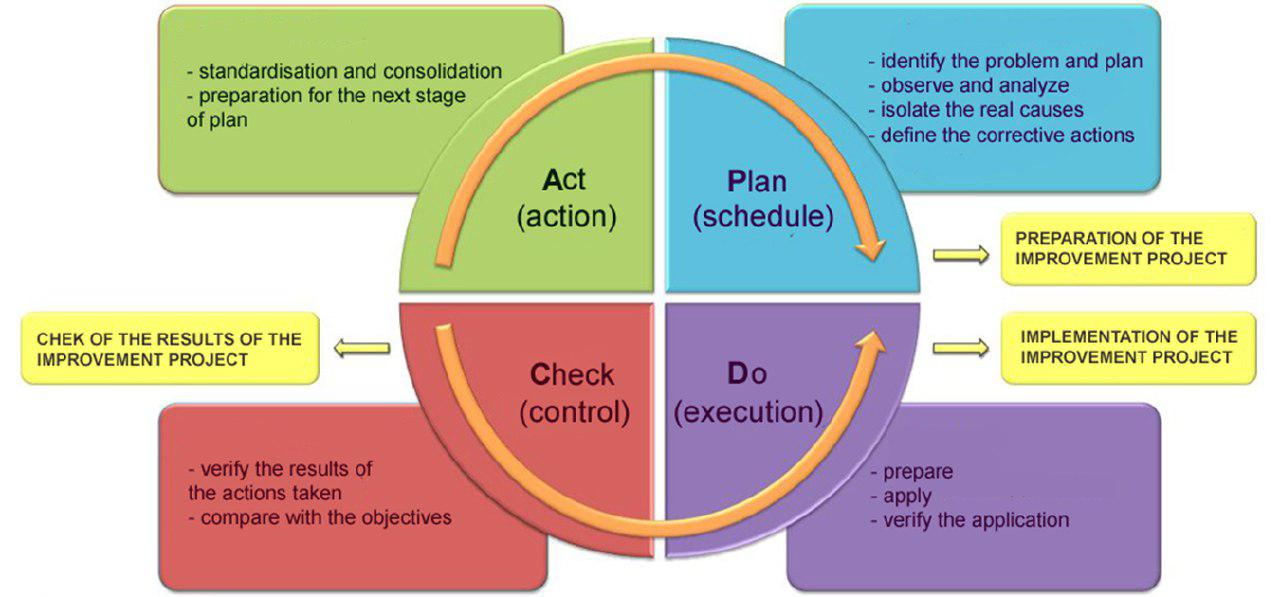
\includegraphics[scale=0.4]{immagini/Pdq/PDCA.png}
					\caption{Fasi del principio PDCA.}
				\end{figure}
			\subsubsection{Qualità di prodotto}
				Al fine di aumentare il valore del prodotto e di migliorarne il funzionamento è necessario fissare degli obbiettivi
				qualitativi e garantire che saranno raggiunti.\\
				Questi obbiettivi sono descritti nell'ISO/IEC 9126 dove sono anche descritte le metriche per misurare gli stessi.\\
				I criteri valutativi sono suddivisi in 3 aree:
				\begin{itemize}
					\item \textbf{Qualità esterna:} Le metriche esterne, specificate nella norma ISO/IEC 9126-2, valutano i
					comportamenti del prodotto sulla base di prove, dall'operatività e dall'osservazione durante la sua esecuzione,
					in funzione degli obiettivi stabiliti.
					\item \textbf{Qualità interna:} È specificata nella norma ISO/IEC 9126-3 e si applica al software non
					eseguibile durante la progettazione e la codifica dello stesso, le misure effettuate consentono di prevedere il
					livello di qualità esterna ed interna, in quanto gli attributi interni influenzano quelli esterni e di uso
					\item \textbf{Qualità d'uso:}  Rappresenta la qualità dal punto di vista dell'utente finale, viene raggiunto
					quando sono raggiunte la qualità esterna e quella interna, le metriche di valutazione sono fornite nella norma
					ISO/IEC 9126-4.
				\end{itemize}
				
				lo standard ISO/IEC 9126 prevede di suddividere la qualità esterna ed interna in 6 caratteristiche principali tra
				le quali la funzionalità è l'unico “requisito funzionale”  mentre le altre 5 sono “requisiti di qualità”, ciascuna
				caratteristica si suddivide in altre sotto caratteristiche che possono essere misurate qualitativamente:
				\begin{itemize}
					\item \textbf{Funzionalità:} capacità del prodotto software di fornire funzioni che rispondano
					a esigenze stabilite
					\begin{itemize}
						\item \textbf{Idoneità:} capacità del prodotto software di fornire un insieme di funzioni per attività
						specifiche già conosciute dall'utente;
						\item \textbf{Accuratezza:} capacità del prodotto software di fornire risultati esatti o concordi al grado di precisione necessario;
						\item \textbf{Interoperabilità:} capacità del prodotto software di interagire con uno o più sistemi 
						precedentemente specificati;
						\item \textbf{Sicurezza:} capacità del prodotto software di proteggere dati e informazioni;
						\item \textbf{Conformità funzionale:} capacità del prodotto software di aderire a standard, convenzioni
						o regolamentazioni e prescrizioni in materia di funzionalità.
					\end{itemize}
					
					\item \textbf{Affidabilità:} capacità del prodotto software di mantenere uno specifico livello di prestazioni
					quando usato
					\begin{itemize}
						\item \textbf{Maturità:} capacità del prodotto software di non fallire a causa di errori nel software;
						\item \textbf{Tolleranza agli errori:} capacità del prodotto software di mantenere un adeguato livello di
						prestazioni e funzioni in caso di errori software o di violazioni;
						\item \textbf{Capacità di recupero:} capacità del prodotto software di ristabilire un adeguato livello di
						performance e di recuperare i dati in caso di errori;
						\item \textbf{Conformità di affidabilità:} capacità del prodotto software di aderire a standard,
						convenzioni o regolamentazioni in materia di affidabilità.
					\end{itemize}										
					
					\item \textbf{Usabilità:} capacità del software di essere capito, imparato, usato e apprezzato dall'utente
					quando usato
					\begin{itemize}
						\item \textbf{Comprensibilità:} capacità del prodotto software di far comprendere all'utente se il
						prodotto è adatto ad uno specifico scopo;
						\item \textbf{Apprendibilità:} capacità del prodotto software di ridurre all'utente il tempo necessario
						per apprendere le sue funzioni;
						\item \textbf{Operabilità:} capacità del prodotto software di essere utilizzato dall'utente in modo
						controllato
						\item \textbf{Attrattiva:} capacità del prodotto software di creare interesse nell'utente;
						\item \textbf{Conformità di usabilità:} capacità del prodotto software di aderire a standard, convenzioni
						o regolamentazioni in materia di usabilità.
					\end{itemize}										
					
					\item \textbf{Efficienza:} capacità del software di fornire prestazioni appropriate in relazione alla quantità
					di risorse in utilizzo
					\begin{itemize}
						\item \textbf{Comportamento temporale:} capacità del software di fornire tempi di risposta e di
						elaborazione adeguati sotto condizioni determinate;
						\item \textbf{Utilizzo di risorse:} capacità del prodotto software di utilizzare quantità e tipo di
						risorse adeguate durante la sua esecuzione;
						\item \textbf{Conformità di efficienza:} capacità del prodotto software di aderire a standard,
						convenzioni o regolamentazioni in materia di efficienza.
					\end{itemize}										
					
					\item \textbf{Manutenibilità:} capacità del prodotto software di essere modificato e ampliato.
					\begin{itemize}
						\item \textbf{Analizzabilità:} rappresenta la facilità con la quale è possibile analizzare il software alla
						ricerca di carenze e difetti;
						\item \textbf{Modificabilità:} capacità del prodotto software di permettere l'implementazione di una
						specifica modifica o di un aggiornamento;
						\item \textbf{Stabilità:} capacità del prodotto software di evitare effetti indesiderati causati da uno o
						più aggiornamenti o modifiche;
						\item \textbf{Testabilità:} capacità del prodotto software di consentire una facile validazione di una
						versione modificata del software;
						\item \textbf{Conformità di manutenibilità:} capacità del prodotto software di aderire a standard,
						convenzioni o regolamentazioni in materia di manutenibilità.
					\end{itemize}										
					
					\item \textbf{Portabilità:} capacità del prodotto software di poter essere trasferito da un ambiente di lavoro
					ad un altro sia dal punto di vista hardware che per quanto riguarda il sistema operativo
					\begin{itemize}
						\item \textbf{Adattabilità:} capacità del prodotto software di essere adattato a diversi ambienti di
						lavoro senza la necessità di effettuare modifiche aggiuntive;
						\item \textbf{Installabilità:} capacità del prodotto software di poter essere installato in specifici
						ambienti;
						\item \textbf{Coesistenza:} capacità del prodotto software di coesistere in ambienti comuni con altri
						software indipendenti condividendo risorse comuni;
						\item \textbf{Sostituibilità:} capacità del prodotto software di poter sostituire un software analogo o
						simile nello stesso ambiente;
						\item \textbf{Conformità di portabilità:} capacità del prodotto software di aderire a standard,
						convenzioni o regolamentazioni in materia di portabilità.
					\end{itemize}										
					
				\end{itemize}
				\begin{figure}[H]
				\centering
					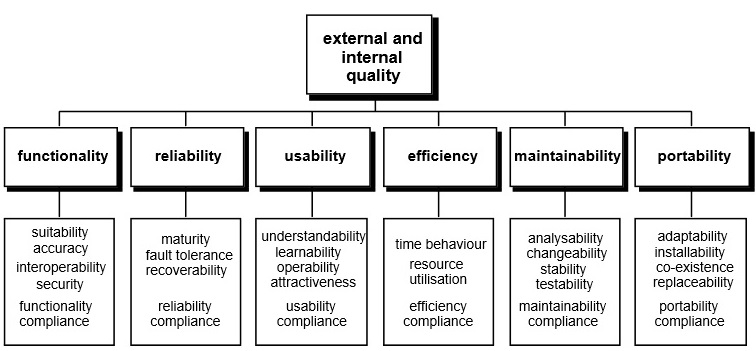
\includegraphics[scale=0.65]{immagini/Pdq/metrichediqualita.png}
					\caption{Caratteristiche della qualità esterna e interna.}
				\end{figure}
				Per la qualità d'uso invece vengono invece definite le seguenti caratteristiche:
				\begin{itemize}
					\item \textbf{Efficacia:} la capacità del prodotto di consentire agli utenti di raggiungere gli obiettivi
					specificati con precisione sufficiente e completezza. 
					\item \textbf{Produttività:} la capacità di consentire agli utenti di utilizzare una quantità di risorse
					appropriate in relazione all'efficacia ottenuta in contesto d'uso definito. 
					\item \textbf{Soddisfazione:} è la capacità del prodotto di soddisfare gli utenti. 
					\item \textbf{Sicurezza:} rappresenta la capacità del prodotto di avere accettabili livelli di rischio per
					quanto riguarda i danni alle persone, al software, ad apparecchiature o all'ambiente operativo d'uso. 
				\end{itemize}
				
				\begin{figure}[H]
					\centering
					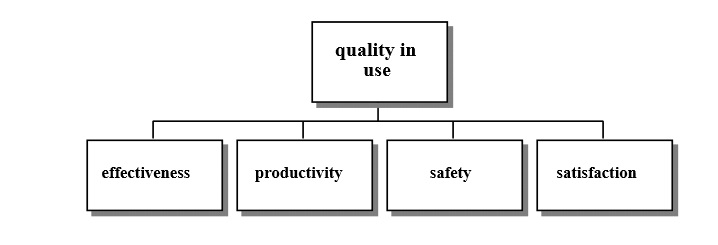
\includegraphics[scale=0.65]{immagini/Pdq/qualitainuso.png}
					\caption{Caratteristiche della qualità d'uso.}
				\end{figure}
				\subsection{Resoconto delle attività di verifica}
				\subsubsection{Riassunto delle attività di verifica}
			Durante la stesura della documentazione sono stati verificati ad ogni modifica sostanziale la documentazione stessa, i
			casi d'uso e i requisiti; è stato in oltre verificato se i processi si sono svolti in maniera corretta.
			\subsubsection{Documentazione}
				I documenti sono stati verificati tramite walkthrough da due persone differenti seguendo il seguente protocollo:
				\begin{itemize}
					\item Verifica della sintassi e della correzione ortografica
					\item Verifica della chiarezza espositiva
					\item Verifica del rispetto delle \emph{Norme Di Progetto v1.1.1} capitolo 3.1
					\item Verifica dell'uniformità dei termini rispetto allo stesso documento
					\item Verifica dell'uniformità dei termini rispetto agli altri documenti
					\item Verifica che i termini che lo necessitano siano stati inseriti nel glossario
					\item Produzione dei un file .txt contenente tutti gli errori al fine di mostrare le correzioni necessarie e
					facilitare la stesura della checklist degli errori più frequenti
				\end{itemize}
				In seguito i documenti sono stati nuovamente verificati tramite inspection utilizzando la checklist precedentemente
				stilata.
			
			\subsubsection{Casi d'uso}
				I casi d'uso sono stati verificati sempre tramite walkthrough ponendo l'attenzione sui seguenti punti:
				\begin{itemize}
					\item Uniformità dei termini usati tra i vari UC
					\item Uniformità tra l'immagine dei diagrammi e la spiegazione della suddetta
					\item Correttezza del codice utilizzato rispetto a quanto definito nelle \emph{Norme Di Progetto v1.1.1} sezione
					2.1.3
					\item Uniformità dei casi d'uso rispetto al capitolato
					\item Rispetto della struttura definita nelle \emph{Norme Di Progetto v1.1.1} sezione 2.3.1
				\end{itemize}

				I Casi d'uso sono stati successivamente ricontrollati all'interno del documento di \emph{Analisi Dei Requisiti} come
				descritto nella sezione 4.2.2
			\subsubsection{Requisiti}
				I requisiti sono stati controllati tramite walkthrough seguendo il seguente protocollo:
					\begin{itemize}
						\item Verifica che la fonte del requisito sia corretta.
						\item Nel caso in cui la fonte sia un UC, verifica che sia l’UC corretto e valutazione
	 sulla possibilità di dedurre altri requisiti dallo stesso.
						\item Verifica uniformità dei termini tra i requisiti.
						\item Rispetto del codice e della struttura definiti nelle \emph{Norme di Progetto v1.1.1} sezione 2.1.2.
						\item I Casi d'uso sono stati successivamente ricontrollati all'interno del documento di \emph{Analisi Dei Requisiti} 
						come descritto in sezione 4.1.
					\end{itemize}
			\subsubsection{Processi}
				I processi sono stati verificati dal responsabile grazie all'utilizzo di teamwork controllando le seguenti condizioni:
				\begin{itemize}
					\item Che la verifica non sia stata effettuata dallo stesso che ha prodotto il materiale da verificare.
					\item Che i documenti siano stati prodotti nell'ordine e nei tempi corretti.
					\item Che le ore di verifica siano almeno 30\% delle ore totali.
					\item Che le riunioni e i brainstorming si siano svolti come definito nelle \emph{Norme di Progetto v1.1.1} sezione 4.2.3.
				\end{itemize}
			\subsubsection{metriche dei documenti}
					\begin{table}[H]
						\begin{tabularx}{\textwidth}{L P P P P P}
							\noalign{\hrule height 1.5pt}
							\rowcolor{orange!85} documenti & Gulpease & parole & figure per pagina & parole per section & errori ortografici\\
							\noalign{\hrule height 1.5pt}
								Norme di progetto & 44,03 & 4180 & 1,61 & 87,08 & 0 \\
							\noalign{\hrule height 0.5pt}
								Studio di fattibilità & 39,84 & 1471 & 0,5 & 49,03 & 0 \\
							\noalign{\hrule height 0.5pt}
								Analisi dei requisiti & 50,32 & 4404 & 2,15 & 38,3 & 0 \\
							\noalign{\hrule height 0.5pt}
								Piano di progetto & 45,01 & 4492 & 2,85 & 56,15 & 0 \\
							\noalign{\hrule height 0.5pt}
								Piano di qualifica & dopo & dopo & dopo & dopo & dopo \\
							\noalign{\hrule height 0.5pt}
								Specifica tecnica & dopo & dopo & dopo & dopo & dopo \\
							\noalign{\hrule height 1.5pt}
						\end{tabularx}
						\caption{Tabella metriche dei documenti }
						\label{SVBVTable}
					\end{table}
				
		\subsection{Tracciamento componenti - requisiti}
		
		\subsection{Dettaglio delle verifiche tramite analisi}
			\subsubsection{Processi}
				Vengono qui di seguito riportate le macro-attività della fase di analisi con associati i relativi valori di SV e BV.
					\begin{table}[H]
						\begin{tabularx}{\textwidth}{m f s X}
							\noalign{\hrule height 1.5pt}
							\rowcolor{orange!85} Macro-attività & SV & BV \\
							\noalign{\hrule height 1.5pt}
								Norme di progetto & ore 1 & \euro \ 30 \\
							\noalign{\hrule height 0.5pt}
								Studio di fattibilità & ore 2 & \euro \ 50 \\
							\noalign{\hrule height 0.5pt}
								Analisi dei requisiti & ore -2 & \euro \ -20 \\
							\noalign{\hrule height 0.5pt}
								Piano di progetto & ore -1 & \euro \ -22 \\
							\noalign{\hrule height 0.5pt}
								Piano di qualifica & ore 0 & \euro \ 0 \\
							\noalign{\hrule height 1.5pt}
						\end{tabularx}
						\caption{Tabella delle attività con SV e BV }
						\label{SVBVTable}
					\end{table}
					
				Da questi dati si può dedurre che:
					\begin{itemize}
						\item I tempi impiegati hanno subito delle leggere variazioni e grazie agli slack inseriti nel 
						\emph{Piano di progetto} non ci sono stati ritardi significativi.
						\item Il costo effettivo è molto vicino a quanto preventivato nel \emph{Piano di progetto} anche se 
						alcuni picchi, specie nello studio di fattibilità, significano che è possibile migliorare la 
						pianificazione dei processi.
					\end{itemize}
			
				Durante la prima fase di analisi le problematiche riscontrate sui processi sono dovute per la maggior parte 
				all'inesperienza del gruppo. A questa fase seguirà una pianificazione su come migliorare i processi che sono 
				risultati più critici.
				
			\subsubsection{Documenti}
			Segue la tabella contenente il valore di tutte le metriche riguardanti i documenti rispetto agli stessi. I valori sono tutti consoni al livello di accettazione definito nella sezione 2.2 .
					\begin{table}[H]
						\begin{tabularx}{\textwidth}{L P P P P P}
							\noalign{\hrule height 1.5pt}
							\rowcolor{orange!85} documenti & Gulpease & parole & figure per pagina & parole per section & errori ortografici\\
							\noalign{\hrule height 1.5pt}
								Norme di progetto & 44,03 & 4180 & 1,61 & 87,08 & 0 \\
							\noalign{\hrule height 0.5pt}
								Studio di fattibilità & 39,84 & 1471 & 0,5 & 49,03 & 0 \\
							\noalign{\hrule height 0.5pt}
								Analisi dei requisiti & 50,32 & 4404 & 2,15 & 38,3 & 0 \\
							\noalign{\hrule height 0.5pt}
								Piano di progetto & 45,01 & 4492 & 2,85 & 56,15 & 0 \\
							\noalign{\hrule height 0.5pt}
								Piano di qualifica & dopo & dopo & dopo & dopo & dopo \\
							\noalign{\hrule height 0.5pt}
								Specifica tecnica & dopo & dopo & dopo & dopo & dopo \\
							\noalign{\hrule height 1.5pt}
						\end{tabularx}
						\caption{Tabella metriche dei documenti }
						\label{SVBVTable}
					\end{table}
	\subsection{Pianificazione dei test}
		Di seguito saranno descritti i test di sistema, integrazione e validazione che sono previsti.
		Nelle tabelle sottostanti la sigla N.E sta per non eseguito.				
	\subsubsection{Test di sistema}
		Viene mostrata di seguito la tabella con tutti i test di sistema che consentono di verificare il sistema rispetto ai requisiti descritti nell'\emph{Analisi dei Requisiti v1.3.11} e la tabella che traccia ogni requisito al test.
		Per ogni comando testato sarà anche verificato il corretto riconoscimento e la corretta gestione degli errori.
		I test di sistema sono nominati per associazione ai casi d'uso.
		\LTXtable{\textwidth}{Tabelle/tabelle_test/test_sistema.tex}
		\LTXtable{\textwidth}{Tabelle/tabelle_test/requisiti_test_sistema.tex}
		
	\subsubsection{Test di integrazione}
		Viene mostrata di seguito la tabella contenente tutti i test di integrazione, atti a verificare il corretto funzionamento delle singole componenti del sistema descritte nella \emph{Specifica Tecnica v1.0.1}. 
		\LTXtable{\textwidth}{Tabelle/tabelle_test/test_integrazione.tex}
			
			\subsection{Lista errori frequenti}
			\begin{itemize}
					\item \textbf{Norme stilistiche:}
					\begin{itemize}
						\item Nome del documento: non viene utilizzata la macro predisposta;
						\item Versione del documento in prima pagina errata;
						\item Immagini mancanti;
						\item Spazi lasciati vuoti per aggiunte successive e non rimossi;
						\item Mancanza di uniformità delle espressioni all'interno dello stesso documento;
						\item Mancanze nella sezione dei riferimenti.
					\end{itemize}
					\item \textbf{Italiano:}
					\begin{itemize}
						\item Doppie;
						\item Accenti.
					\end{itemize}
					\item \textbf{\LaTeX :}
					\begin{itemize}
						\item mancanza dell'indice delle immagini e delle tabelle.
					\end{itemize}
					\item \textbf{UML:}
					\begin{itemize}
						\item incongruenze tra l'immagine contenente i diagrammi e la descrizione testuale della stessa;
						\item errori nel testo delle immagini dovute a copia-incolla.
					\end{itemize}
				\end{itemize}
				
\cleardoublepage
	\addcontentsline{toc}{chapter}{\listfigurename}
	\listoffigures
	
	\cleardoublepage
	\addcontentsline{toc}{chapter}{\listtablename}
	\listoftables	
\end{document}
